\documentclass[aspectratio=169]{beamer}

\mode<presentation> {
\usetheme{SimplePlus} 
\usecolortheme{dolphin}
\setbeamertemplate{navigation symbols}{}
}

\usepackage{graphicx} 
\usepackage{booktabs} 
\usepackage[export]{adjustbox}
\usepackage{blindtext}
\usepackage{hyperref}
\usepackage{amssymb}
\usepackage{amsmath}
\usepackage{bbm}
\usepackage{pgfplots}
\usetikzlibrary{intersections}
\pgfplotsset{compat=1.16}
\usepackage{tikz}
\usetikzlibrary{arrows.meta}
\usepackage[round]{natbib}
\bibliographystyle{apalike}
\usepackage{multirow,array}
\usepackage{threeparttable}
\usepackage[dvipsnames]{xcolor}
\usepackage[T1]{fontenc}\usepackage{lmodern}
\newcommand{\sym}[1]{\ifmmode^{#1}\else\(^{#1}\)\fi}


\title[Informality and financial conditions]{\Huge \textbf{Informality and financial conditions}} 

\author[Morales \& Puggioni]{\textbf{David Morales} \inst{1} \and \textbf{Daniela Puggioni} \inst{2}}
\institute[TSE \and Banxico]{ \inst{1} \textbf{Toulouse School of Economics} \\
david.morales@tse-fr.eu \and 
\inst{2} \textbf{Bank of Mexico}} 

\date[September 17, 2026] 
{\large \textbf{BID Job-Markle Seminar}\\
September 17, 2026}

\begin{document}

%------------------------------------------------
\begin{frame}[noframenumbering] 
\titlepage
\end{frame}

%------------------------------------------------

\begin{frame}{The link between informality and financial conditions}
\label{motivation}

\begin{columns}
    \begin{column}{0.3\textwidth} 
        \onslide<1->{\textbf{\textcolor{BrickRed}{Informality}}:}    
        \onslide<1->{\begin{itemize}
            \item Prevalent across time and regions.
            \item Implications on tax collection, inequality, etc.
            \item Failed policies, e.g. special tax regimes (RIF, REPECO, etc).
        \end{itemize}
        \vspace{3mm}
        \onslide<2->{\textbf{This paper}:
        \begin{itemize}
            \item Financial conditions? 
        \end{itemize}}}
    \end{column}
    
    \begin{column}{0.7\textwidth} 
        \onslide<2->{\begin{center}
            \includegraphics[scale=0.43]{slides_material/fig_crosscountry_informality.png}
        \end{center}}
    \end{column}
\end{columns}

\vspace{3mm}

\onslide<1->{\textcolor{BrickRed}{\textbf{Informal}}: A firm with positive revenue and workers but no Social Security contributions.} 

\hyperlink{maintransition}{\beamergotobutton{Informality transitions}} \qquad \qquad \hyperlink{intensive}{\beamergotobutton{Intensive margin}} \qquad \qquad \hyperlink{imss}{\beamergotobutton{IMSS employer number}} \qquad \qquad \hyperlink{rfc}{\beamergotobutton{RFC tax number}} 

\end{frame}

%------------------------------------------------


\begin{frame}{This paper} \label{this_paper}

\begin{center}
    \Large \textbf{RQ}: Is formality sensitive to financial conditions?
\end{center}

\vspace{2mm}
\pause

\textbf{Answer}
\begin{itemize}
    \item Yes! Credit terms can reallocate firms and resources towards the formal sector.
\end{itemize}

\vspace{1mm}
\pause

\textbf{Method}
\begin{itemize}
    \item Leave-One-Out Shift-Share IV (LOO-SSIV) with exogenous shift.
    \item Dynamic model of firm transitions with sector-specific financial constraints.
\end{itemize}

\vspace{1mm}
\pause

\textbf{Why it matters}
\begin{itemize}
    \item Financial development increases formalization, w/ more efficient resource allocation.
\end{itemize}

\vspace{1mm}
\pause

\textbf{Contribution}
\begin{itemize}
    \item First causal evidence that bank credit supply shocks increase firm formalization.
    \item $\uparrow$ Credit $\Rightarrow$ $\downarrow$ Capital constraints $\Rightarrow$ $\uparrow$ Formal entry \& formalization $\Rightarrow$ $\downarrow$ Informality.
\end{itemize}

\end{frame}

%------------------------------------------------

\begin{frame}[noframenumbering]{Outline}

\Large

1) Literature

\vspace{3mm}

\textcolor{lightgray}{2) Data}

\vspace{3mm}

\textcolor{lightgray}{3) Empirical Strategy}

\vspace{3mm}

\textcolor{lightgray}{4) Results}

\vspace{3mm}

\textcolor{lightgray}{5) Model}

\vspace{3mm}

\textcolor{lightgray}{6) Estimation}

\vspace{3mm}

\textcolor{lightgray}{7) Counterfactuals}

\vspace{3mm}

\textcolor{lightgray}{8) Conclusions}


\end{frame}

%------------------------------------------------

\begin{frame}{Literature}\label{literature}
Credit supply effects on firm activity \textcolor{lightgray}{\citep{khwaja2008tracing,chodorow2014employment,amiti2018much,greenstone2020credit,gutierrez2023credit}, etc.}
 \begin{itemize}
    \item \textbf{Literature takeaway}: Credit affects only formal employment and investment.
    \item \textbf{Contribution}: Credit also affects informal firms through the formalization margin.
 \end{itemize}
\vspace{8mm}
\pause
Informality: causes and consequences \textcolor{lightgray}{\citep{la2014informality,meghir2015wages,busso2012formal,almeida2012enforcement,ulyssea2018firms,adom2025structural}, etc.}
\begin{itemize}
    \item \textbf{Literature takeaway}: No firm dynamics, formality as an absorbing state.
     \item \textbf{Contribution}: Full dynamics, entry, exit, and switching in both directions.
 \end{itemize}
\vspace{8mm}
\pause
\begin{itemize}
    \centering
    \item[$\Rightarrow$] \Large \textbf{This paper}: Formality is (also) a financing decision.
\end{itemize}
\end{frame}

%------------------------------------------------

\begin{frame}[noframenumbering]{Outline}

\Large

\textcolor{lightgray}{1) Literature}

\vspace{3mm}

2) Data

\vspace{3mm}

\textcolor{lightgray}{3) Empirical Strategy}

\vspace{3mm}

\textcolor{lightgray}{4) Results}

\vspace{3mm}

\textcolor{lightgray}{5) Model}

\vspace{3mm}

\textcolor{lightgray}{6) Estimation}

\vspace{3mm}

\textcolor{lightgray}{7) Counterfactuals}

\vspace{3mm}

\textcolor{lightgray}{8) Conclusions}


\end{frame}

%------------------------------------------------

\begin{frame}{Data}\label{data}

\textbf{Mexican data}

\vspace{3mm}

\begin{itemize}
    \item Matched bank--employer--employee data \textcolor{gray}{Social Security (IMSS) + National Banking and Securities Commission (CNBV)}
    \begin{itemize}
        \item 2005--2025: monthly credit registry, annual market panel.
        \item Universe of formal employers and workers.
        \item Universe of business loans to formal and informal firms.
    \end{itemize}
    \vspace{3mm}
    \pause
    
    \item Economic Census \textcolor{gray}{(EC)}
    \begin{itemize}
        \item Every 5 years (2009, 2014, 2019, \& 2024).
        \item Formal and informal establishments: entry, exit, and five-year formality transitions.
    \end{itemize}
    \vspace{3mm}
    \pause
    
    \item Coverage: 703 markets = commuting zones, 119 banks, and 3.3 m. borrower firms.
\end{itemize}
\vspace{3mm}
\pause

\begin{center}
    \large \textbf{Key feature:} Credit + formality + firm dynamics observed in the same markets.
\end{center}

\end{frame}

%------------------------------------------------

\begin{frame}[noframenumbering]{Outline}

\Large

\textcolor{lightgray}{1) Literature}

\vspace{3mm}

\textcolor{lightgray}{2) Data}

\vspace{3mm}

3) Empirical Strategy

\vspace{3mm}

\textcolor{lightgray}{4) Results}

\vspace{3mm}

\textcolor{lightgray}{5) Model}

\vspace{3mm}

\textcolor{lightgray}{6) Estimation}

\vspace{3mm}

\textcolor{lightgray}{7) Counterfactuals}

\vspace{3mm}

\textcolor{lightgray}{8) Conclusions}


\end{frame}

%------------------------------------------------

\begin{frame}{\textbf{Empirical strategy}: Leave-One-Out Shift-Share IV, LOO-SSIV} \label{iv_market_level}

\textbf{Intuition}: Each bank's credit supply growth (estimated nationally w/multi-bank firms, excluding target market) weighted by that bank's initial lending share in the target market.

\vspace{5mm}
\pause

\textbf{1) Decompose demand and supply}: Regress bank-market credit on bank and firm FE:

\begin{equation*}
     \Delta \ln L_{bft}^{-m} = \alpha_{ft}^{-m} + \gamma_{bt}^{-m} + \epsilon_{bft}, \quad \quad \Rightarrow \quad \quad \hat{\gamma}_{b,t}^{-m} = \text{Exogenous shift.} 
\end{equation*}
\pause

\textbf{2) Share}: Banks' share of total loans in a market at baseline:

\begin{equation*}
    s_{b,m,t-1} = \frac{L_{b,m,t-1}}{\sum_b L_{b,m,t-1}}, \quad \quad \Rightarrow \quad \quad s_{b,m,t-1} = \text{Identifying variation.} 
\end{equation*}
\pause

\textbf{3) Instrument}: Bank change in credit supply weighted by market share.  
% \hyperlink{iv_bank_level}{\beamergotobutton{Shock}}

\begin{equation*}
    \hat{Z}_{m,t}^{LOO} = \sum_b \left( s_{b,m,t-1} \times \hat{\gamma}_{b,t}^{-m} \right) 
\end{equation*}

% \begin{center}
%     \Large \textbf{Interpretation}: Different exposure of markets to exogenous bank shocks.
% \end{center}

\end{frame}

%------------------------------------------------

\begin{frame}[noframenumbering]{Outline}

\Large

\textcolor{lightgray}{1) Literature}

\vspace{3mm}

\textcolor{lightgray}{2) Data}

\vspace{3mm}

\textcolor{lightgray}{3) Empirical Strategy}

\vspace{3mm}

4) Results

\vspace{3mm}

\textcolor{lightgray}{5) Model}

\vspace{3mm}

\textcolor{lightgray}{6) Estimation}

\vspace{3mm}

\textcolor{lightgray}{7) Counterfactuals}

\vspace{3mm}

\textcolor{lightgray}{8) Conclusions}


\end{frame}

%------------------------------------------------

\begin{frame}{The identifying variation across local markets}
\label{maps}

\begin{columns}
    \begin{column}{0.5\textwidth} 
        \begin{center}
            \includegraphics[scale=0.14]{slides_material/map_iv.png}\\
            {\small \textbf{Instrument}}
        \end{center}
    \end{column}

    \begin{column}{0.5\textwidth} 
        \begin{center}
            \includegraphics[scale=0.14]{slides_material/map_informality.png}\\
            {\small \textbf{Informality share}}
        \end{center}
    \end{column}
\end{columns}

\vspace{3mm}

\textbf{Takeaway}: IV varies across markets and it is unrelated to baseline informality.

\vspace{3mm}

\hfill \hyperlink{creditmap}{\beamergotobutton{Credit change map}}

\end{frame}

%------------------------------------------------

\begin{frame}{The instrument is relevant}

\begin{columns}
    \begin{column}{0.6\textwidth} 
        \begin{center}
            \includegraphics[scale=0.21]{slides_material/first_stage.png}
        \end{center}
    \end{column}

    \begin{column}{0.4\textwidth} 
        \begin{itemize}
            \item +1  s.d. IV doubles credit (+4.4 M USD, median mkt).
            \vspace{3mm}
            \item Relevant: 1st stage F = 307.
            \vspace{3mm}
            \item Effective Nb. of banks $\approx$ 10 $\Rightarrow$ Concentrated but no single bank drives results. 
        \end{itemize}
    \end{column}
    
\end{columns}

\begin{center}
    \large \textbf{Interpretation}: Shocks capture supply variation, but where does this shock go? 
\end{center}

\end{frame}

%------------------------------------------------

\begin{frame}{A credit supply shock deepens more than it widens}

\textbf{What does a 10\% credit supply shock imply?}

\begin{itemize}
    \item + 455 thousand USD in the median market (Median credit = 4.5 million USD).
\end{itemize}

\pause
\vspace{5mm}

\textbf{Where does this credit go?}

\begin{itemize}
    \item 84\% (382 thousand USD) to existing borrowers (more and bigger credits).
    \item 16\% (73 thousand USD) to new borrowers, + 11 new firms borrowing per market. 
\end{itemize}

\[
\underbrace{+10\%}_{\text{Market credit}} \;=\; \underbrace{6.4\%^{***}}_{\text{Loan size}} \;+\;
\underbrace{2.0\%^{***}}_{\text{Loans p/borrower}} \;+\;
\underbrace{1.6\%^{***}}_{\text{New borrowers}} 
\]

\vspace{5mm}

\begin{center}
    \large \textbf{Supply shock}: more loans for existing borrowers and few new firms at the margin.
\end{center}
\end{frame}

%------------------------------------------------

\begin{frame}{A credit supply shock affects collateral more than pricing}

\textbf{Collateral}: The median market collateral requires 16 centavos per peso lent.
\begin{itemize}
    \item A 10\% credit supply expansion reduces the collateral requirement 17\%, from 16 to 13 centavos per peso (elasticity $-1.86^{***}$).
\end{itemize}

\pause
\vspace{5mm}

\textbf{Interest rate}: The average market interest rate is 15.0\%.
\begin{itemize}
    \item A + 10\% credit supply expansion moves it 4 basis points, from 15.00\% to 15.04\%.
    \item Within bank re-pricing, no reallocation towards cheaper banks.
    \begin{itemize}
        \item Consistent with banks reaching marginally riskier borrowers.
    \end{itemize}
\end{itemize}

\vspace{5mm}
\pause

\begin{center}
    \large \textbf{Mechanism}: Credit supply moves the collateral, not the price.
\end{center}

\end{frame}

%------------------------------------------------

\begin{frame}{More credit generates firm reallocation \& formal firm creation}

\begin{columns}[T] 
    \begin{column}{0.6\textwidth} 
        \begin{center}
        \vspace{-5mm}
            \includegraphics[scale=0.19]{slides_material/decomp.png}
        \end{center}
    \end{column}

    \begin{column}{0.4\textwidth} 
        \vspace{5mm}
        A supply driven $\uparrow 10\%$ mkt credit:
        \begin{itemize}
            \item \textbf{Entry}: +3 (+1,965 national) formal firms.
            \item \textbf{Exit}: +1.4 (+917) formal \& +15 (+9,825) informal firms.
            \item \textbf{Transitions}: +1.6 (+1,048) formalization, -1.1 (-721) in-formalization.
        \end{itemize}
        \vspace{5mm}
        \pause
    \end{column}
\end{columns}

\vspace{3mm}

\textbf{Relevant start-up rate}: +0.24 p.p. vs. - 0.78 trend in USA \textcolor{gray}{\cite{pugsley2019grown}}.

\pause
\vspace{3mm}

\textbf{VS tax cut:} $+3.4\%$ formal firms vs halving Brazil's tax ($+4.3\%$) \textcolor{gray}{\citep{rocha2018lower}}

\end{frame}

%------------------------------------------------

\begin{frame}{Credit rises formal employment \& reduces informal production}

\begin{center}
    {\small
    \begin{threeparttable}
        \begin{tabular}{lccccc}
            \toprule
             & \multicolumn{3}{c}{Formal labor market (IMSS)} & \multicolumn{2}{c}{Value added (census)} \\
            \cmidrule(lr){2-4} \cmidrule(lr){5-6}
             & Employment & Wage bill & Avg.\ wage & Informal & Total \\
            \midrule
            $\Delta_5 \ln(\text{credit})$ & 0.019$^{***}$ & 0.023$^{**}$ & $-$0.012$^{***}$ & $-$0.052$^{**}$ & 0.030$^{*}$ \\
             & (0.005) & (0.009) & (0.004) & (0.022) & (0.016) \\
            \addlinespace
            Mean dep.\ var. & 30{,}695 & \$0.66m & \$10.7 & \$0.30bn & \$1.17bn \\
            Observations             & 1{,}382  & 1{,}382 & 1{,}382 & 1{,}390 & 1{,}390 \\
            \bottomrule
        \end{tabular}
        \begin{tablenotes}[flushleft]
            \tiny
            \item Means are levels on each column's sample, in USD at 19 MXN/USD. Controls: employment- and credit-weighted sectoral \\
            composition, lagged market rate, log banks, log credits, uncovered share, bank share, coverage $\times$ year. AKM s.e. in parenthesis.
        \end{tablenotes}
    \end{threeparttable}
    }
\end{center}
\pause

\vspace{3mm}

\textbf{Credit moves the formal worker margin where enacted tax reforms did not} 
\begin{itemize}
    \item $\approx 0$ on Mexico's border VAT halving \textcolor{gray}{\cite{campos2020effects}}.
    \item $\approx 0$ on revenue neutral payroll reforms \textcolor{gray}{\cite{bobba2021labor}}.
\end{itemize}

\pause

\vspace{3mm}

\textbf{Less productive average informal firm}: Marginal most productive ones became formal.

\end{frame}

%------------------------------------------------

\begin{frame}{Robustness checks}\label{robustness}

\begin{enumerate}
    \item \textbf{Balance Test}: IV's residual variation $\perp$ predetermined characteristics. \hyperlink{balance}{\beamergotobutton{Go}}
    \vspace{1mm}
    \pause
    \item \textbf{OLS, Reduced form}: Effect without invoking IV decomposition. \hyperlink{ols}{\beamergotobutton{Go}}
    \vspace{1mm}
    \pause
    \item \textbf{Wo/3 biggest metropolitan areas}: Effects valid out of metropolitan areas. \hyperlink{womet}{\beamergotobutton{Go}}
    \vspace{1mm}
    \pause
    \item \textbf{Unweighted}: Conclusions not artifact of credit weighting. \hyperlink{unweighted}{\beamergotobutton{Go}}
    \vspace{1mm}
    \pause
    \item \textbf{Placebo test}: Absence of pre-trends. \hyperlink{placebo}{\beamergotobutton{Go}}
    \vspace{1mm}
    \pause
    \item \textbf{Drop largest bank}: Effects not driven by a single bank. \hyperlink{dropbank}{\beamergotobutton{Go}}
    \vspace{1mm}
    \pause
    \item \textbf{Conventional non-LOO}: Same results. \hyperlink{nonloo}{\beamergotobutton{Go}}
    \vspace{1mm}
    \pause
    \item \textbf{Bank level}: Surprisingly similar elasticities, it also considers uni-bank firms. \hyperlink{banklevel}{\beamergotobutton{Go}}
    \vspace{1mm}
    \pause
    \item \textbf{Different coverages}: Similar effects. \hyperlink{coverage}{\beamergotobutton{Go}}
\end{enumerate}

\begin{center}
    \Large Consistent evidence of credit driven formalization.
\end{center}
\pause

But which mechanisms? Tax avoidance, capital constraints, or productivity selection? $\cdots$ 

\begin{center}
    \Large \textbf{Model}
\end{center}

\end{frame}

%------------------------------------------------

\begin{frame}[noframenumbering]{Outline}

\Large

\textcolor{lightgray}{1) Literature}

\vspace{3mm}

\textcolor{lightgray}{2) Data}

\vspace{3mm}

\textcolor{lightgray}{3) Empirical Strategy}

\vspace{3mm}

\textcolor{lightgray}{4) Results}

\vspace{3mm}

5) Model

\vspace{3mm}

\textcolor{lightgray}{6) Estimation}

\vspace{3mm}

\textcolor{lightgray}{7) Counterfactuals}

\vspace{3mm}

\textcolor{lightgray}{8) Conclusions}


\end{frame}

%------------------------------------------------

\begin{frame}{Settings, simplified model version (two periods)}

\begin{columns}[T]
    \column{0.52\textwidth}
    \textbf{Technology and heterogeneity}
    \begin{itemize}
        \item $y=\theta k^{\alpha}\ell^{\nu}$, $\alpha+\nu<1$.
        \item $\ln\theta_{1}=\ln v+u_{1}$.
        $\ln\theta_{2}=\rho\ln\theta_{1}+(1-\rho)\ln v+u_{2}$.
        \begin{itemize}
            \item $\Pi_s(x,k) = c x k^{\alpha/(1-\nu)}$, \quad $x\equiv\theta^{\frac{1}{1-\nu}}$
            \pause
        \end{itemize}
    \end{itemize}
    \textbf{Fiscal side}
    \begin{itemize}
      \item Formal, s = f: revenue $\tau_y$ \& payroll tax $\tau_l$
      \item Informal, s = i: evades both.
      \pause
    \end{itemize}
    \textbf{Assumptions}
    \begin{itemize}
        \item Partial Eq.: w exogenous.
        \item Mkt: Prices \& goods formal = informal
        \pause
    \end{itemize}
    
    \column{0.44\textwidth}
    \textbf{Within period loans}
    \begin{itemize}
        \item Cost: $\Phi_{s}(a)=r_{s} \times a$, \quad $r_{i}>r_{f}$.
        \item Collateral: $a\leq b_{s}k'$, \quad
        $b_{i}<b_{f}$.
        \item Internal funds: n
        \item Borrowing: $ a = (k'-n)^{+} \le b_s k'$
        \pause
    \end{itemize}
    \textbf{Costs}
    \begin{itemize}
      \item Entry fees: $C^e_{s}$, \quad $C^e_{f} > C^e_{i}$.
      \item Switch fees: $C_{if}, C_{fi}$.
      \item Fixed cost: $C_{i} < C_{f}$.
      \item Exogenous death: $\lambda_{s}$, depreciation: $\delta$, \& discounted: $\beta$.
      \pause
    \end{itemize}
\end{columns}

\bigskip
\textbf{Timing:} Decisions, before $u_2$ observed, based on expected productivity $\hat{x} = \mathbb{E} \big[x_{2}\mid\theta_{1},v\big]$.

\end{frame}
 
% ---------------------------------------------------------------

\begin{frame}\label{value_functions}
\frametitle{Value functions} \label{valuefunctions}

\begin{align*}
    \text{\textbf{Entrant}}: & V^{e}(k_0,\hat{x}) = \max\Big\{ \underbrace{k_0}_{\text{\textcolor{gray}{Stay out}}} \,,\; \underbrace{W_i\big(k_0 - C^{e}_{i},\hat{x}\big)}_{\text{\textcolor{BrickRed}{Enter informal}}} \,,\; \underbrace{W_f\big(k_0 - C^{e}_{f},\hat{x}\big)}_{\text{\textcolor{RoyalBlue}{Enter formal}}} \Big\} \quad \hyperlink{operatingvalue}{\beamergotobutton{$W_s(n,\hat x)$}}
\end{align*}
\pause

\begin{align*}
    \text{\textbf{Informal incumbent}}: & V_i(k,\hat{x}) = \max\Big\{ \underbrace{(1-\delta)k}_{\text{\textcolor{gray}{Exit}}} \,,\; \underbrace{W_i\big((1-\delta)k,\hat{x}\big)}_{\text{\textcolor{BrickRed}{Stay informal}}} \,,\; \underbrace{W_f\big((1-\delta)k - C_{if},\hat{x}\big)}_{\text{\textcolor{RoyalBlue}{Formalize}}} \Big\}
\end{align*}
\pause

\begin{align*}
    \text{\textbf{Formal incumbent}}: & V_f(k,\hat{x}) = \max\Big\{ \underbrace{(1-\delta)k}_{\text{\textcolor{gray}{Exit}}} \,,\; \underbrace{W_f\big((1-\delta)k,\hat{x}\big)}_{\text{\textcolor{RoyalBlue}{Stay formal}}} \,,\; \underbrace{W_i\big((1-\delta)k - C_{fi},\hat{x}\big)}_{\text{\textcolor{BrickRed}{De-formalize}}} \Big\}
\end{align*}
\pause

\vspace{3mm}

\begin{center}
    \large \textbf{Sector decision}: Firms choose the status that maximizes lifetime value.
\end{center}


\end{frame}

%------------------------------------------------

\begin{frame}{Unique threshold decision rules}\label{threshold}

There exists a unique threshold for each transition: $ \hat x_i^X < \hat x_i^E < \hat x_f^X < \hat x_f^I < \hat x_f^E < \hat x_i^F $.

\begin{center}
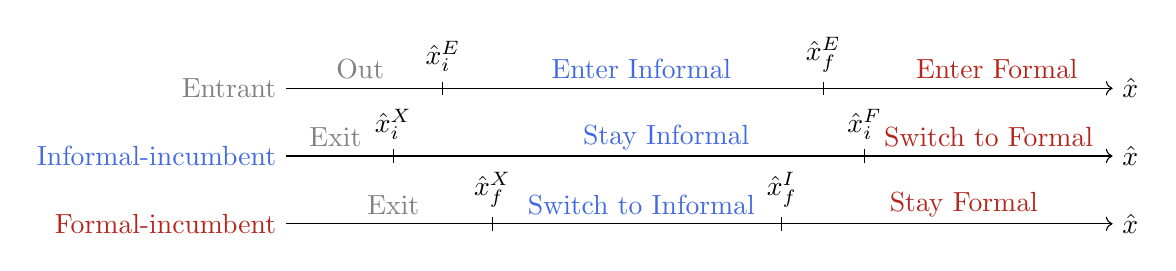
\begin{tikzpicture}[xscale=1.05, yscale=0.86, every node/.style={font=\normalsize}]
  % entrant line
  \draw[->] (0,2) -- (10,2) node[right] {$\hat x$};
  \node[left] at (0,2) {\textcolor{gray}{Entrant}};
  \foreach \x/\lab in {1.9/{$\hat x_i^E$}, 6.5/{$\hat x_f^E$}}
    \draw (\x,1.9) -- (\x,2.1) node[above] {\lab};
  \node at (0.9,2.28) {\textcolor{gray}{Out}};
  \node at (4.3,2.28) {\textcolor{RoyalBlue}{Enter Informal}};
  \node at (8.6,2.28) {\textcolor{BrickRed}{Enter Formal}};
  % informal incumbent
  \draw[->] (0,1) -- (10,1) node[right] {$\hat x$};
  \node[left] at (0,1) {\textcolor{RoyalBlue}{Informal-incumbent}};
  \foreach \x/\lab in {1.3/{$\hat x_i^X$}, 7.0/{$\hat x_i^F$}}
    \draw (\x,0.9) -- (\x,1.1) node[above] {\lab};
  \node at (0.6,1.28) {\textcolor{gray}{Exit}};
  \node at (4.6,1.28) {\textcolor{RoyalBlue}{Stay Informal}};
  \node at (8.5,1.28) {\textcolor{BrickRed}{Switch to Formal}};
  % formal incumbent
  \draw[->] (0,0) -- (10,0) node[right] {$\hat x$};
  \node[left] at (0,0) {\textcolor{BrickRed}{Formal-incumbent}};
  \foreach \x/\lab in {2.5/{$\hat x_f^X$}, 6.0/{$\hat x_f^I$}}
    \draw (\x,-0.1) -- (\x,0.1) node[above] {\lab};
  \node at (1.3,0.28) {\textcolor{gray}{Exit}};
  \node at (4.3,0.28) {\textcolor{RoyalBlue}{Switch to Informal}};
  \node at (8.2,0.28) {\textcolor{BrickRed}{Stay Formal}};
\end{tikzpicture}
\end{center}

\vspace{5mm}

\textbf{Financial conditions?}: Thresholds depend on finance for constrained firms, $\hat x_s^{S}(r_s,b_s)$.

\vspace{5mm}

\textbf{But who are the constrained firms}?

\vspace{3mm}

\hyperlink{formalthresholdcf}{\beamergotobutton{Formality threshold closed form}} \qquad \hyperlink{entryexitthresholdcf}{\beamergotobutton{Entry-Exit threshold closed form}}

\end{frame}
 
% ----------------------------------------------------------------------

\begin{frame}{Investment and financing: a four-region policy}

\[
\text{\textbf{Optimal capital}} =
\begin{cases}
    \bar{k}_{s}
    \Leftarrow \mathrm{MPK}
    = 1-\beta(1-\delta) \equiv \mathrm{MCK}
    & \text{if no borrowing.} \\[6pt]
    \tilde{k}_{s}
    \Leftarrow \mathrm{MPK}
    = 1-\beta(1-\delta)+r_s \equiv \mathrm{MCK}
    & \text{if borrowing.}
\end{cases}
\]

\vspace{3mm}

\begin{center}
    \renewcommand{\arraystretch}{1.25}\small
    \begin{tabular}{lllll}
        \toprule
         Region & Funds ($n$) vs. $k^{*}_{s}$ & Capital $k^{*}_{s}$ &
         Borrowing $a^{*}_{s}$ & Cash-flow sens.\ \\
        \midrule
        1: Unconstrained & $n\geq\bar k_{s}$ & $\bar k_{s}(\hat{x})$
         & 0 & 0 \\
        2: No borrow, low k & $\tilde k_{s}\leq n<\bar k_{s}$ &
         $n$ & 0 & 1 \\
        3: Borrower & $(1-b_{s})\tilde k_{s}\leq n
         <\tilde k_{s}$ & $\tilde k_{s}(\hat{x})$ & $\tilde k_{s}-n$
         & 0 \\
        4: Collateral-capped & $n<(1-b_{s})\tilde k_{s}$ &
         $\dfrac{n}{1-b_{s}}$ & $b_{s}k^{*}_{s}$ &
         $\dfrac{1}{1-b_{s}}$ \\
        \bottomrule
    \end{tabular}
\end{center}

\vspace{2mm}
\pause

\structure{Takeaway:} Credit shocks affect only firms in region 3 and 4.

\vspace{2mm}
\pause

\textbf{Three model channels}: Tax avoidance, capital constraints, and productivity selection.

\end{frame}
 
% ----------------------------------------------------

\begin{frame}[noframenumbering]{Outline}

\Large

\textcolor{lightgray}{1) Literature}

\vspace{3mm}

\textcolor{lightgray}{2) Data}

\vspace{3mm}

\textcolor{lightgray}{3) Empirical Strategy}

\vspace{3mm}

\textcolor{lightgray}{4) Results}

\vspace{3mm}

\textcolor{lightgray}{5) Model}

\vspace{3mm}

6) Estimation

\vspace{3mm}

\textcolor{lightgray}{7) Counterfactuals}

\vspace{3mm}

\textcolor{lightgray}{8) Conclusions}


\end{frame}

%------------------------------------------------

\begin{frame}{Estimation}\label{estimation}

\begin{enumerate}
    \item \textbf{Institutional}: 
    \begin{itemize}
        \item Discount factor ($\beta=0.95$, standard). 
        \item Depreciation rate ($\delta=0.10$, standard). 
        \item Effective taxes ($\tau_y=0.05$ \& $\tau_\ell=0.16$, tax authority).
    \end{itemize}
    \vspace{4mm}\pause
    \item \textbf{Estimated outside the model}: 
    \begin{itemize}
        \item K \& L weights ($\alpha=0.17$ \& $\nu=0.59$, Census cost shares).
        \item Exogenous death rates ($\lambda_i=0.067$ \& $\lambda_f=0.056$, size flat exit tail).
        \item TFP process ($\rho_i=0.95$, $\rho_f=0.95$, $\sigma_v=0.56$, sector specific innovations).
        \item Lending spreads ($r_i=0.11$ \& $r_f=0.024$, rates over risk-free rate).
        \item Collateral limits ($b_i=0.85$ < $b_f=0.90$, P90 leverage).
        \item Informality detection scale ($\eta_i=2.71$, labor share gap).
    \end{itemize}
    \vspace{4mm}\pause
    \item \textbf{15 Core parameters}: Model estimated, next slide.
\end{enumerate}

\end{frame}

%------------------------------------------------

\begin{frame}{Estimation: GMM on cross-section \& credit-supply responses}

\textbf{15 parameters jointly estimated}: 

\begin{columns}
    \begin{column}{0.5\textwidth} 
        \begin{itemize}
            \item Operating fixed cost ($C_i$ \& $C_f$).
            \item Entry cost ($C^e_i$ \& $C^e_f$).
            \item Transition cost ($C_{if}$ \& $C_{fi}$).
            \item Financial fixed cost ($C^b_i$ \& $C^b_f$).
        \end{itemize}
    \end{column}

    \begin{column}{0.5\textwidth} 
        \begin{itemize}
            \item Entrant wealth ($\mu_{k0}$ \& $\sigma_{k0}$).
            \item Formality taste shock ($\sigma_c$).
            \item Shock incidence ($\chi_i, \chi_f, \kappa_i, \& \kappa_f$).
        \end{itemize}
    \end{column}
\end{columns}

\vspace{10mm}\pause

\textbf{23 moments}; Overidentified with 8 df.
\begin{itemize}
    \item \textbf{10 Cross-section and dynamics}: exit, switching, and entry rates; formal entry share; borrowing incidence; \& entrant capital.
    \item \textbf{13 Credit-supply IV responses}: Stocks, entry, exit, and switching number of (formal \& informal) firms; average and total VA; and collateral.
\end{itemize}

\end{frame}
%------------------------------------------------

\begin{frame}{Identification: each parameter has a leading moment}
\begin{center}
\small
\begin{tabular}{ll}
\toprule
\textbf{Parameter} & \textbf{Leading moment} \\
\midrule
Operating fixed cost $C_i,\, C_f$            & 5-yr exit rate, by sector \\
Entry cost, informal $C^e_i$                  & entrant size relative to incumbents \\
Entry cost, formal $C^e_f$                  & formal share of entrants \\
Formality taste shock $\sigma_c$ \& transition cost $C_{if}$ & 5-yr i$\to$f switch rates \\
Transition cost $C_{fi}$ & 5-yr f$\to$i switch rates \\
Financial fixed cost $C^b_i,\, C^b_f$ & borrowing incidence, by sector \\
Entrant wealth $\mu_{k_0},\, \sigma_{k_0}$ & entrant capital: mean and p90  \\
Shock incidence $\chi_s,\, \kappa_s$ & first stage  \& collateral responses \\
\bottomrule
\end{tabular}
\end{center}
\vspace{2mm}
\textbf{Why}: Monotone comparative statics pair each parameter with its moment.

\begin{itemize}
    \item The sensitivity matrix \textcolor{gray}{(Andrews-Gentzkow-Shapiro)} confirms it.
\end{itemize}

\end{frame}

%------------------------------------------------

\begin{frame}{GMM: Algorithm}

\textbf{Step 0}: Fix the parameters estimated outside the model, guess the 15 remaining.
\vspace{5mm}

\textbf{Loop}: repeat until the Sum of Squared Errors (SSE) stops improving.
\begin{enumerate}
    \item Solve the firm's problem: policies and the stationary distribution (fixed point).
    \item Financial shock ($r_s \to r_s(1 - \chi_s)$ \& $b_s \to b_s(1 + \kappa_s)$), re-solve, and read model $\beta$'s.
    \item Residuals $\big(\frac{m^{model} - \hat m}{\hat m},\; \frac{\beta^{model} - \hat \beta}{\mathrm{s.e.}_{AKM}}\big)$
          $\Rightarrow$ SSE.
    \item Numerical Jacobian: nudge each parameter, record change \textcolor{gray}{(2 solves per parameter)}.
    \item Damped Gauss--Newton step (Levenberg--Marquardt: shrink step if the SSE worsens).
\end{enumerate}

\end{frame}

%------------------------------------------------

\begin{frame}{Model cost parameter estimates}

\begin{center}
    \includegraphics[scale=0.48]{slides_material/fig_theta_costs_B.png}
\end{center}

\textbf{Friction}: Formality is a cost wall, only firms that expect scale pay it.
\begin{itemize}
    \item Operating costs $\times$17(\$62k vs \$3.6k a year), Bank access costs $\times$66 (\$106k vs \$1.6k).  
\end{itemize}

\end{frame}

%------------------------------------------------

\begin{frame}{Model wealth parameter estimates}

\begin{center}
    \includegraphics[scale=0.5]{slides_material/fig_theta_wealth_B.png}
\end{center}

\textbf{Friction}: Initial wealth determines borrowing and formality status.
\begin{itemize}
    \item The median entrant starts with \$820 vs \$62k a year formality operating bill.
\end{itemize}

\end{frame}

%------------------------------------------------

\begin{frame}{Model pass through parameter estimates}
\label{theta}

\begin{center}
    \includegraphics[scale=0.5]{slides_material/fig_theta_incidence_B.png}
\end{center}

\textbf{Mechanism}: A bank supply shock arrives through cheaper formal loan pricing.

\hyperlink{jacobian}{\beamergotobutton{Jacobian}} \quad \hyperlink{sensitivity}{\beamergotobutton{Sensitivity}} \quad \hyperlink{policy}{\beamergotobutton{Policy Partition}}

\end{frame}

%------------------------------------------------

\begin{frame}{Model fit on targeted moments}

\begin{center}
    \includegraphics[scale=0.5]{slides_material/fig_fit_core_levels_B.png}
\end{center}

\textbf{Poor fit}: Gross transitions and borrowing incidence.
\begin{itemize}
    \item \textbf{Reason}: Financial parameters are formality dependent, not firm dependent.
\end{itemize}

\end{frame}

%------------------------------------------------


\begin{frame}{Model fit on IV elasticities}

\begin{center}
    \includegraphics[scale=0.48]{slides_material/fig_fit_coefplot.png}
\end{center}

\textbf{Poor fit}: three out of twelve, exit margins and collateral.
\begin{itemize}
    \item \textbf{Reason}: No GE competition on exits \& collateral is hard, not a negotiated loan term.
\end{itemize}

\end{frame}

%------------------------------------------------

\begin{frame}{Validation, non targeted moments}

\begin{center}
    \includegraphics[scale=0.5]{slides_material/fig_validation_untargeted_B.png}
\end{center}

\textbf{Takeaway}: Model predicts that credit shifts VA towards formal firms as formality rises.
\begin{itemize}
    \item The data validates the model prediction, untargeted. 
\end{itemize}

\end{frame}

%------------------------------------------------

\begin{frame}[noframenumbering]{Outline}

\Large

\textcolor{lightgray}{1) Literature}

\vspace{3mm}

\textcolor{lightgray}{2) Data}

\vspace{3mm}

\textcolor{lightgray}{3) Empirical Strategy}

\vspace{3mm}

\textcolor{lightgray}{4) Results}

\vspace{3mm}

\textcolor{lightgray}{5) Model}

\vspace{3mm}

\textcolor{lightgray}{6) Estimation}

\vspace{3mm}

7) Counterfactuals

\vspace{3mm}

\textcolor{lightgray}{8) Conclusions}


\end{frame}

%------------------------------------------------

\begin{frame}{Counterfactual}
\label{maincounterfactual}

\begin{center}
    \includegraphics[scale=0.5]{slides_material/fig_counterfactuals_B.png} \quad \hyperlink{secondcounterfactual}{\beamergotobutton{+ Variables}}
\end{center}

\textbf{Takeaway 1}: The wall is the financial fixed cost $\Rightarrow$ Two ways to increase formality,
\begin{enumerate}
    \item Reduce the formal financial fixed cost, which increases output.
    \item Increase the informal financial fixed cost, which reduces output.
\end{enumerate}

\textbf{Takeaway 2}: Small tax effect, as in \textcolor{gray}{\citep{bobba2021labor, campos2020effects}}.


\end{frame}

%------------------------------------------------

\begin{frame}[noframenumbering]{Outline}

\Large

\textcolor{lightgray}{1) Literature}

\vspace{3mm}

\textcolor{lightgray}{2) Data}

\vspace{3mm}

\textcolor{lightgray}{3) Empirical Strategy}

\vspace{3mm}

\textcolor{lightgray}{4) Results}

\vspace{3mm}

\textcolor{lightgray}{5) Model}

\vspace{3mm}

\textcolor{lightgray}{6) Estimation}

\vspace{3mm}

7) Counterfactuals

\vspace{3mm}

\textcolor{lightgray}{8) Conclusions}


\end{frame}

%------------------------------------------------

\begin{frame}{Limitations}

\textbf{Empirics}
\begin{itemize}
    \item Causal design is market level: firm level mechanisms come through the model.
\end{itemize}

\vspace{2mm}
\textbf{Model}
\begin{itemize}
    \item No GE displacement (fixed wage, no competition) $\Rightarrow$ exit responses missed.
    \item Collateral is a hard cap, not a negotiated loan term $\Rightarrow$ collateral response missed.
    \item Financial parameters are not firm level
    $\Rightarrow$ transitions \& borrowing incidence missed.
    \item Inference is conditional on calibrated inputs.
\end{itemize}
\end{frame}

%------------------------------------------------

\begin{frame}
\frametitle{\textbf{Conclusions}} \label{conclusion}

\textbf{This paper} $\cdots$

\vspace{4mm}

\begin{itemize}
    \item Documents rich firm dynamics and credit market conditions.
    \begin{itemize}
        \item Formal status is not an absorbing state: + 1/3 of formal firms slide back to informality.
        \item Credit is lightly collateralized (16\%) and its growth is 2/3 incumbents \& 1/3 new. 
    \end{itemize}
    \vspace{2mm}
    \item Causally establishes that credit supply reallocates activity
    toward formality.
    \begin{itemize}
        \item Cheaper credit terms: Collateral -17\% per $+10\%$ credit, rates barely move.
        \item + formal, + formal entry, \& + upward switching;
        - downward switching; +formal VA.
    \end{itemize}
    \vspace{2mm}
    \item Model's mechanism: Formality is a fixed cost wall.
    \begin{itemize}
        \item \$62k/yr to operate and \$106k to
        borrow formally, vs.\ \$3.6k and \$1.6k informally.
        \item Untargeted moments validation: Model's VA
        reallocation prediction confirmed by data.
    \end{itemize}
    \vspace{2mm}
    \item Quantifies policy menu: Financial access is the only tool that formalizes and grows.
    \begin{itemize}
        \item $\downarrow$ formal credit fixed cost: $+3.7$pp formal share,
        $+5.8\%$ VA, $+29\%$ credit ($\approx \times 4$ tax).
        \item Repressing informal credit formalizes ($+2.5$pp) but burns
        $3.9\%$ of output.
    \end{itemize}
\end{itemize}

\end{frame}

%------------------------------------------------

\begin{frame}[noframenumbering]
\centering
\Huge Thank you

\vspace{10mm}

\Large david.morales@tse-fr.eu

\end{frame}

%------------------------------------------------

\begin{frame}[noframenumbering]
\frametitle{\textbf{References}} 

\tiny

\bibliography{ref}

\end{frame}

%------------------------------------------------

\appendix

%------------------------------------------------

\begin{frame}[noframenumbering]{Main transition matrix}\label{maintransition}

\begin{center}
    \includegraphics[scale=0.49]{slides_material/t_mat_ss.png}
\end{center}

\hyperlink{motivation}{\beamergotobutton{Back}}

\end{frame}

%------------------------------------------------

\begin{frame}[noframenumbering]{Transition matrix taking into account the intensive margin}\label{intensive}

\begin{center}
    \includegraphics[scale=0.49]{slides_material/t_mat_ss_mix.png}
\end{center}

\hyperlink{motivation}{\beamergotobutton{Back}}

\end{frame}

%------------------------------------------------

\begin{frame}[noframenumbering]{Transition matrix, IMSS employer number defines informal}\label{imss}

\begin{center}
    \includegraphics[scale=0.55]{slides_material/t_mat_imss.png}
\end{center}

\hyperlink{motivation}{\beamergotobutton{Back}}

\end{frame}

%------------------------------------------------

\begin{frame}[noframenumbering]{Transition matrix, RFC tax number defines informal}\label{rfc}

\begin{center}
    \includegraphics[scale=0.55]{slides_material/t_mat_rfc.png}
\end{center}

\hyperlink{motivation}{\beamergotobutton{Back}}

\end{frame}

%------------------------------------------------

\begin{frame}[noframenumbering]{Five year credit change across markets}\label{creditmap}

\begin{center}
    \includegraphics[scale=0.2]{slides_material/map_credit.png}
\end{center}

\hyperlink{maps}{\beamergotobutton{Back}}

\end{frame}

%------------------------------------------------

\begin{frame}[noframenumbering]
\frametitle{\textbf{Balance test}} \label{balance}
\begin{center}
    \footnotesize
    \begin{tabular}{lcccc}
        \toprule
        & \multicolumn{2}{c}{\textbf{Lagged 5 years}} & \multicolumn{2}{c}{\textbf{Lagged 10 years}} \\
        \cmidrule(lr){2-3} \cmidrule(lr){4-5}
        \textit{Predetermined variable} & $\widehat{\beta}$ & SE & $\widehat{\beta}$ & SE \\
        \midrule
        Market employment share, sector 1     & \phantom{$-$}0.040 & (0.026) & \phantom{$-$}0.038 & (0.027) \\
        Market employment share, sector 2     & $-$0.007 & (0.011) & $-$0.011 & (0.012) \\
        Bank-portfolio sector share, sector 1 & $-$0.007 & (0.031) & \phantom{$-$}0.028 & (0.053) \\
        Bank-portfolio sector share, sector 2 & \phantom{$-$}0.010 & (0.034) & $-$0.057 & (0.061) \\
        Credit-weighted interest rate         & \phantom{$-$}0.330 & (0.258) & \phantom{$-$}0.760 & (0.809) \\
        Log number of banks in market         & $-$0.040 & (0.072) & $-$0.072 & (0.069) \\
        Log number of credits in market       & \phantom{$-$}0.206 & (0.312) & $-$0.038 & (0.316) \\
        Loan-weighted default probability     & $-$4.209 & (2.856) & \multicolumn{2}{c}{---} \\
        Log credit per loan                   & $-$0.683\sym{***} & (0.097) & $-$0.199 & (0.127) \\
        \midrule
        Observations (range)              & \multicolumn{2}{c}{531--1{,}435} & \multicolumn{2}{c}{766--937} \\
        Markets (range)                   & \multicolumn{2}{c}{521--588} & \multicolumn{2}{c}{457--530} \\
        \bottomrule
    \end{tabular}
\end{center}
{\tiny Only credit per loan fails: mechanical mean reversion in the composition of the endogenous credit variable, discussed in text. Default probability exists from 2019 (single window; no 10-year lag).}\\
\hyperlink{robustness}{\beamergotobutton{Back}}
\end{frame}
%------------------------------------------------
\begin{frame}[noframenumbering]
\frametitle{\textbf{OLS estimates}} \label{ols}
\begin{center}
    \scriptsize
    \begin{tabular}{lcr}
        \toprule
        \textit{Dependent variable (log)} & OLS coefficient & $N$ \\
        \midrule
        \multicolumn{3}{l}{\textit{Panel A: Stock and gross flows of firms}} \\
        Number of existing firms --- Total       & \phantom{$-$}0.006          (0.006) & 1{,}390 \\
        Number of existing firms --- Formal      & \phantom{$-$}0.029\sym{**}  (0.013) & 1{,}385 \\
        Number of existing firms --- Informal    & \phantom{$-$}0.003          (0.006) & 1{,}390 \\
        Firm entry --- Total                     & \phantom{$-$}0.014          (0.011) & \phantom{1{,}}992 \\
        Firm entry --- Formal                    & \phantom{$-$}0.038\sym{**}  (0.018) & \phantom{1{,}}975 \\
        Firm entry --- Informal                  & \phantom{$-$}0.012          (0.012) & \phantom{1{,}}992 \\
        Firm exit --- Total                      & \phantom{$-$}0.035\sym{***} (0.007) & \phantom{1{,}}992 \\
        Firm exit --- Formal                     & \phantom{$-$}0.028\sym{**}  (0.012) & \phantom{1{,}}961 \\
        Firm exit --- Informal                   & \phantom{$-$}0.039\sym{***} (0.008) & \phantom{1{,}}992 \\
        \midrule
        \multicolumn{3}{l}{\textit{Panel B: Formality transitions}} \\
        Formal--Formal                           & \phantom{$-$}0.032\sym{**}  (0.015) & \phantom{1{,}}966 \\
        Informal--Formal                         & \phantom{$-$}0.039\sym{**}  (0.018) & \phantom{1{,}}953 \\
        Formal--Informal                         & $-$0.015                    (0.014) & \phantom{1{,}}954 \\
        Informal--Informal                       & \phantom{$-$}0.003          (0.007) & \phantom{1{,}}992 \\
        \bottomrule
    \end{tabular}
\end{center}
{\tiny OLS of the five-year log change on $\Delta_5\ln(\text{credit})$, same controls and weights; s.e.\ clustered by market.}\\
\hyperlink{robustness}{\beamergotobutton{Back}}
\end{frame}
%------------------------------------------------
\begin{frame}[noframenumbering]
\frametitle{\textbf{Without three biggest metropolitan areas}} \label{womet}
\begin{center}
    \scriptsize
    \begin{tabular}{lccr}
        \toprule
        \textit{Dependent variable} & $\widehat{\Delta_5\ln(\text{credit})}$ & First-stage $F$ & $N$ \\
        \midrule
        \multicolumn{4}{l}{\textit{Panel A: Stock and gross flows of firms}} \\
        Log existing firms --- Total    & $-$0.003                    (0.006) & 91.66  & 1{,}381 \\
        Log existing firms --- Formal   & \phantom{$-$}0.049\sym{***} (0.014) & 91.65  & 1{,}376 \\
        Log existing firms --- Informal & $-$0.009                    (0.007) & 91.66  & 1{,}381 \\
        Log firm entry --- Total        & \phantom{$-$}0.018          (0.014) & 119.35 & \phantom{1{,}}986 \\
        Log firm entry --- Formal       & \phantom{$-$}0.067\sym{***} (0.020) & 119.33 & \phantom{1{,}}969 \\
        Log firm entry --- Informal     & \phantom{$-$}0.015          (0.015) & 119.35 & \phantom{1{,}}986 \\
        Log firm exit --- Total         & \phantom{$-$}0.041\sym{**}  (0.018) & 119.35 & \phantom{1{,}}986 \\
        Log firm exit --- Formal        & \phantom{$-$}0.067\sym{***} (0.018) & 119.27 & \phantom{1{,}}955 \\
        Log firm exit --- Informal      & \phantom{$-$}0.037\sym{**}  (0.018) & 119.35 & \phantom{1{,}}986 \\
        \midrule
        \multicolumn{4}{l}{\textit{Panel B: Formality transitions}} \\
        Formal--Formal                  & \phantom{$-$}0.055\sym{***} (0.009) & 119.28 & \phantom{1{,}}960 \\
        Informal--Formal                & \phantom{$-$}0.014          (0.020) & 118.67 & \phantom{1{,}}947 \\
        Formal--Informal                & $-$0.048\sym{**}            (0.023) & 119.25 & \phantom{1{,}}948 \\
        Informal--Informal              & $-$0.025\sym{***}           (0.006) & 119.35 & \phantom{1{,}}986 \\
        \bottomrule
    \end{tabular}
\end{center}
{\tiny AKM exposure-robust s.e.; stars from AKM $p$-values.}\\
\hyperlink{robustness}{\beamergotobutton{Back}}
\end{frame}
%------------------------------------------------
\begin{frame}[noframenumbering]
\frametitle{\textbf{Unweighted regression}} \label{unweighted}
\begin{center}
    \scriptsize
    \begin{tabular}{lccr}
        \toprule
        \textit{Dependent variable} & $\widehat{\Delta_5\ln(\text{credit})}$ & First-stage $F$ & $N$ \\
        \midrule
        \multicolumn{4}{l}{\textit{Panel A: Stock and gross flows of firms}} \\
        Log existing firms --- Total    & \phantom{$-$}0.022 (0.029) & 34.86 & 1{,}390 \\
        Log existing firms --- Formal   & \phantom{$-$}0.064 (0.080) & 40.97 & 1{,}385 \\
        Log existing firms --- Informal & \phantom{$-$}0.021 (0.032) & 34.86 & 1{,}390 \\
        Log firm entry --- Total        & \phantom{$-$}0.067 (0.086) & 26.04 & \phantom{1{,}}992 \\
        Log firm entry --- Formal       & \phantom{$-$}0.090 (0.167) & 38.41 & \phantom{1{,}}975 \\
        Log firm entry --- Informal     & \phantom{$-$}0.066 (0.095) & 26.04 & \phantom{1{,}}992 \\
        Log firm exit --- Total         & \phantom{$-$}0.017 (0.120) & 26.04 & \phantom{1{,}}992 \\
        Log firm exit --- Formal        & $-$0.048           (0.246) & 30.07 & \phantom{1{,}}961 \\
        Log firm exit --- Informal      & \phantom{$-$}0.027 (0.143) & 26.04 & \phantom{1{,}}992 \\
        \midrule
        \multicolumn{4}{l}{\textit{Panel B: Formality transitions}} \\
        Formal--Formal                  & \phantom{$-$}0.102 (0.248) & 29.55 & \phantom{1{,}}966 \\
        Informal--Formal                & \phantom{$-$}0.053 (0.327) & 51.97 & \phantom{1{,}}953 \\
        Formal--Informal                & \phantom{$-$}0.064 (0.450) & 39.31 & \phantom{1{,}}954 \\
        Informal--Informal              & $-$0.006           (0.072) & 26.04 & \phantom{1{,}}992 \\
        \bottomrule
    \end{tabular}
\end{center}
{\tiny AKM exposure-robust s.e.\ widen by an order of magnitude without credit weights (small rural markets dominate); point estimates preserve the pattern.}\\
\hyperlink{robustness}{\beamergotobutton{Back}}
\end{frame}
%------------------------------------------------
\begin{frame}[noframenumbering]
\frametitle{\textbf{Placebo test}} \label{placebo}
\begin{center}
    \scriptsize
    \begin{tabular}{lccr}
        \toprule
        \textit{Pre-period outcome ($\Delta_5 Y_{t-5}$, log)} & $\widehat{\Delta_5\ln(\text{credit})}$ & 1st-stage $F$ & $N$ \\
        \midrule
        \multicolumn{4}{l}{\textit{Panel A: Stock and gross flows of firms}} \\
        Number of existing firms --- Total      & \phantom{$-$}0.016\sym{***} (0.005) & 346.22 & \phantom{1{,}}979 \\
        Number of existing firms --- Formal     & \phantom{$-$}0.017\sym{**}  (0.008) & 346.15 & \phantom{1{,}}975 \\
        Number of existing firms --- Informal   & \phantom{$-$}0.019\sym{***} (0.006) & 346.22 & \phantom{1{,}}979 \\
        Firm entry --- Total                    & \phantom{$-$}0.030          (0.106) & 2.59   & \phantom{1{,}}512 \\
        Firm entry --- Formal                   & $-$0.065                    (0.242) & 2.59   & \phantom{1{,}}506 \\
        Firm entry --- Informal                 & \phantom{$-$}0.041          (0.094) & 2.59   & \phantom{1{,}}512 \\
        Firm exit --- Total                     & $-$0.038                    (0.110) & 2.59   & \phantom{1{,}}512 \\
        Firm exit --- Formal                    & \phantom{$-$}0.122          (0.294) & 2.59   & \phantom{1{,}}493 \\
        Firm exit --- Informal                  & $-$0.070                    (0.102) & 2.59   & \phantom{1{,}}512 \\
        \midrule
        \multicolumn{4}{l}{\textit{Panel B: Formality transitions}} \\
        Formal--Formal                          & $-$0.015                    (0.066) & 2.26   & \phantom{1{,}}486 \\
        Informal--Formal                        & $-$0.093                    (0.171) & 2.59   & \phantom{1{,}}494 \\
        Formal--Informal                        & \phantom{$-$}0.060          (0.169) & 2.59   & \phantom{1{,}}483 \\
        Informal--Informal                      & $-$0.040                    (0.103) & 2.59   & \phantom{1{,}}512 \\
        \bottomrule
    \end{tabular}
\end{center}
{\tiny Stock rows use the full panel ($F=346$); lagged flow changes exist only in one overlapping census window ($F=2.6$, uninformative by construction). Controlling for the lagged own change, the small stock coefficients vanish (0.003 and $-$0.002, ns) while the formal-stock effect stands (0.048\sym{***}).}\\
\hyperlink{robustness}{\beamergotobutton{Back}}
\end{frame}
%------------------------------------------------
\begin{frame}[noframenumbering]
\frametitle{\textbf{Dropping the largest bank}} \label{dropbank}
\begin{center}
    \scriptsize
    \begin{tabular}{lccr}
        \toprule
        \textit{Dependent variable} & $\widehat{\Delta_5\ln(\text{credit})}$ & First-stage $F$ & $N$ \\
        \midrule
        \multicolumn{4}{l}{\textit{Panel A: Stock and gross flows of firms}} \\
        Log existing firms --- Total    & \phantom{$-$}0.000          (0.006) & 32.17 & 1{,}390 \\
        Log existing firms --- Formal   & \phantom{$-$}0.048\sym{***} (0.010) & 32.17 & 1{,}385 \\
        Log existing firms --- Informal & $-$0.006                    (0.008) & 32.17 & 1{,}390 \\
        Log firm entry --- Total        & \phantom{$-$}0.004          (0.011) & 31.54 & \phantom{1{,}}992 \\
        Log firm entry --- Formal       & \phantom{$-$}0.058\sym{***} (0.012) & 31.54 & \phantom{1{,}}975 \\
        Log firm entry --- Informal     & \phantom{$-$}0.001          (0.013) & 31.54 & \phantom{1{,}}992 \\
        Log firm exit --- Total         & \phantom{$-$}0.046\sym{***} (0.016) & 31.54 & \phantom{1{,}}992 \\
        Log firm exit --- Formal        & $-$0.000                    (0.017) & 31.53 & \phantom{1{,}}961 \\
        Log firm exit --- Informal      & \phantom{$-$}0.061\sym{***} (0.016) & 31.54 & \phantom{1{,}}992 \\
        \midrule
        \multicolumn{4}{l}{\textit{Panel B: Formality transitions}} \\
        Formal--Formal                  & \phantom{$-$}0.030\sym{***} (0.009) & 31.53 & \phantom{1{,}}966 \\
        Informal--Formal                & \phantom{$-$}0.093\sym{***} (0.021) & 31.73 & \phantom{1{,}}953 \\
        Formal--Informal                & $-$0.078\sym{***}           (0.025) & 31.53 & \phantom{1{,}}954 \\
        Informal--Informal              & \phantom{$-$}0.000          (0.004) & 31.54 & \phantom{1{,}}992 \\
        \bottomrule
    \end{tabular}
\end{center}
{\tiny Instrument rebuilt excluding the bank with the largest exposure weight (26.8\% of exposure weights). First stage 0.97 (0.17); decomposition identities hold exactly. AKM s.e.}\\
\hyperlink{robustness}{\beamergotobutton{Back}}
\end{frame}
%------------------------------------------------
\begin{frame}[noframenumbering]
\frametitle{\textbf{Conventional non-LOO estimates}} \label{nonloo}
\begin{center}
    \scriptsize
    \begin{tabular}{lccr}
        \toprule
        \textit{Dependent variable} & $\widehat{\Delta_5\ln(\text{credit})}$ & First-stage $F$ & $N$ \\
        \midrule
        \multicolumn{4}{l}{\textit{Panel A: Stock and gross flows of firms}} \\
        Log existing firms --- Total    & \phantom{$-$}0.001          (0.005) [0.960] & 264.47 & 1{,}390 \\
        Log existing firms --- Formal   & \phantom{$-$}0.036\sym{***} (0.008) [0.046] & 264.42 & 1{,}385 \\
        Log existing firms --- Informal & $-$0.002                    (0.006) [0.917] & 264.47 & 1{,}390 \\
        Log firm entry --- Total        & \phantom{$-$}0.007          (0.009) [0.781] & 272.77 & \phantom{1{,}}992 \\
        Log firm entry --- Formal       & \phantom{$-$}0.043\sym{***} (0.010) [0.136] & 272.58 & \phantom{1{,}}975 \\
        Log firm entry --- Informal     & \phantom{$-$}0.006          (0.010) [0.806] & 272.77 & \phantom{1{,}}992 \\
        Log firm exit --- Total         & \phantom{$-$}0.049\sym{***} (0.009) [0.003] & 272.77 & \phantom{1{,}}992 \\
        Log firm exit --- Formal        & \phantom{$-$}0.023          (0.018) [0.433] & 272.58 & \phantom{1{,}}961 \\
        Log firm exit --- Informal      & \phantom{$-$}0.060\sym{***} (0.008) [0.000] & 272.77 & \phantom{1{,}}992 \\
        \midrule
        \multicolumn{4}{l}{\textit{Panel B: Formality transitions}} \\
        Formal--Formal                  & \phantom{$-$}0.027\sym{***} (0.004) [0.138] & 272.51 & \phantom{1{,}}966 \\
        Informal--Formal                & \phantom{$-$}0.050\sym{**}  (0.020) [0.101] & 271.75 & \phantom{1{,}}953 \\
        Formal--Informal                & $-$0.044\sym{***}           (0.013) [0.289] & 272.53 & \phantom{1{,}}954 \\
        Informal--Informal              & $-$0.003                    (0.003) [0.869] & 272.77 & \phantom{1{,}}992 \\
        \bottomrule
    \end{tabular}
\end{center}
{\tiny Non-leave-one-out shift-share; corr with the LOO instrument 0.9998 (credit-weighted). AKM s.e.; wild-bootstrap $p$ in brackets.}\\
\hyperlink{robustness}{\beamergotobutton{Back}}
\end{frame}
%------------------------------------------------
\begin{frame}[noframenumbering]
\frametitle{\textbf{Bank level estimation}} \label{banklevel}
\begin{center}
    \scriptsize
    \begin{tabular}{lccr}
        \toprule
        \textit{Dependent variable} & $\widehat{\Delta_5\ln(\text{credit})}$ & First-stage $F$ & $N$ \\
        \midrule
        \multicolumn{4}{l}{\textit{Panel A: Stock and gross flows of firms}} \\
        Log existing firms --- Total     & $-$0.004                    (0.005) [0.588] & 34.91 & 131 \\
        Log existing firms --- Formal    & \phantom{$-$}0.036\sym{***} (0.008) [0.000] & 34.91 & 131 \\
        Log existing firms --- Informal  & $-$0.009\sym{*}             (0.005) [0.188] & 34.91 & 131 \\
        Log firm entry --- Total         & $-$0.001                    (0.008) [0.959] & 30.40 & 105 \\
        Log firm entry --- Formal        & \phantom{$-$}0.045\sym{***} (0.011) [0.001] & 30.40 & 105 \\
        Log firm entry --- Informal      & $-$0.004                    (0.009) [0.771] & 30.40 & 105 \\
        Log firm exit --- Total          & \phantom{$-$}0.058\sym{***} (0.011) [0.004] & 30.40 & 105 \\
        Log firm exit --- Formal         & \phantom{$-$}0.020          (0.016) [0.320] & 30.40 & 105 \\
        Log firm exit --- Informal       & \phantom{$-$}0.070\sym{***} (0.010) [0.000] & 30.40 & 105 \\
        \midrule
        \multicolumn{4}{l}{\textit{Panel B: Formality transitions}} \\
        Formal--Formal                   & \phantom{$-$}0.021\sym{***} (0.008) [0.062] & 30.40 & 105 \\
        Informal--Formal                 & \phantom{$-$}0.068\sym{***} (0.013) [0.000] & 30.40 & 105 \\
        Formal--Informal                 & $-$0.077\sym{***}           (0.015) [0.008] & 30.40 & 105 \\
        Informal--Informal               & $-$0.003                    (0.004) [0.699] & 30.40 & 105 \\
        \bottomrule
    \end{tabular}
\end{center}
{\tiny S.e.\ clustered by bank (67 banks; 66 in the flow sample); wild-bootstrap $p$ in brackets.}\\
\hyperlink{robustness}{\beamergotobutton{Back}}
\end{frame}
%------------------------------------------------
\begin{frame}[noframenumbering]
\frametitle{\textbf{Different coverages}} \label{coverage}
\begin{center}
    \tiny
    \begin{tabular}{lcccccccc}
        \toprule
        & \multicolumn{4}{c}{\textbf{Coverage $\geq$ 0}}
        & \multicolumn{4}{c}{\textbf{Coverage $\geq$ 0.8}} \\
        \cmidrule(lr){2-5} \cmidrule(lr){6-9}
        \textit{Dependent variable}
        & $\hat\beta$ (s.e.) & $F$ & $N$ & $M$
        & $\hat\beta$ (s.e.) & $F$ & $N$ & $M$ \\
        \midrule
        \multicolumn{9}{l}{\textit{Panel A: Stock and gross flows of firms}} \\
        Log existing firms --- Total
        & $-$0.000 (0.005) & 124.21 & 1{,}520 & 568
        & 0.003 (0.005) & 284.48 & 1{,}215 & 541 \\
        Log existing firms --- Formal
        & 0.042\sym{***} (0.009) & 124.22 & 1{,}514 & 564
        & 0.045\sym{***} (0.012) & 284.42 & 1{,}210 & 537 \\
        Log existing firms --- Informal
        & $-$0.005 (0.006) & 124.21 & 1{,}520 & 568
        & $-$0.001 (0.006) & 284.48 & 1{,}215 & 541 \\
        Log firm entry --- Total
        & 0.009 (0.008) & 121.56 & 1{,}092 & 568
        & 0.012 (0.010) & 321.21 & \phantom{1{,}}859 & 525 \\
        Log firm entry --- Formal
        & 0.058\sym{***} (0.013) & 121.54 & 1{,}071 & 555
        & 0.058\sym{***} (0.016) & 320.85 & \phantom{1{,}}843 & 514 \\
        Log firm entry --- Informal
        & 0.006 (0.009) & 121.56 & 1{,}091 & 568
        & 0.010 (0.009) & 321.21 & \phantom{1{,}}859 & 525 \\
        Log firm exit --- Total
        & 0.040\sym{***} (0.009) & 121.56 & 1{,}092 & 568
        & 0.047\sym{***} (0.012) & 321.21 & \phantom{1{,}}859 & 525 \\
        Log firm exit --- Formal
        & 0.017 (0.011) & 121.69 & 1{,}049 & 549
        & 0.032\sym{**} (0.013) & 321.03 & \phantom{1{,}}831 & 508 \\
        Log firm exit --- Informal
        & 0.047\sym{***} (0.010) & 121.56 & 1{,}092 & 568
        & 0.056\sym{***} (0.013) & 321.21 & \phantom{1{,}}859 & 525 \\
        \midrule
        \multicolumn{9}{l}{\textit{Panel B: Formality transitions}} \\
        Formal--Formal
        & 0.018\sym{***} (0.007) & 122.28 & 1{,}051 & 553
        & 0.034\sym{***} (0.008) & 320.91 & \phantom{1{,}}834 & 511 \\
        Informal--Formal
        & 0.058\sym{***} (0.014) & 120.08 & 1{,}042 & 540
        & 0.051\sym{***} (0.017) & 319.38 & \phantom{1{,}}824 & 498 \\
        Formal--Informal
        & $-$0.060\sym{***} (0.016) & 121.73 & 1{,}040 & 541
        & $-$0.034\sym{**} (0.014) & 320.90 & \phantom{1{,}}826 & 503 \\
        Informal--Informal
        & $-$0.008\sym{*} (0.004) & 121.56 & 1{,}091 & 568
        & $-$0.005 (0.004) & 321.21 & \phantom{1{,}}859 & 525 \\
        \bottomrule
    \end{tabular}
\end{center}
{\tiny AKM exposure-robust s.e.; stars from AKM $p$-values.}\\
\hyperlink{robustness}{\beamergotobutton{Back}}
\end{frame}
%------------------------------------------------

\begin{frame}[noframenumbering]
\frametitle{\textbf{Operating value}} \label{operatingvalue}

\textbf{Operating value}

\[
W_s(n,\hat{x}) = \max_{k'}\Big\{
\underbrace{n - k' - \Phi_s(a)}_{\text{dividend today}}
+ \beta \Big[ \underbrace{(1-\delta)k'}_{\text{scrap}}
+ (1-\lambda_s)\underbrace{\big(\Pi_s(\hat{x},k') - C_s\big)}_{\text{produce if alive}} \Big]\Big\}
\]

\hyperlink{valuefunctions}{\beamergotobutton{Back}}

\end{frame}

%-----------------------------------------------

\begin{frame}[noframenumbering]{The formality margin: single crossing}
\label{formalthresholdcf} 

For origin $o$ (entrant, i-incumbent, f-incumbent) with funds $n_{o}$, on the borrowing region the formal-vs-informal comparison is \emph{affine} in $\hat x^{1/(1-\gamma)}$:

\begin{equation*}
  \Delta_{o}(\hat x)=A\,\hat x^{\frac{1}{1-\gamma}}
  -B\,n_{o}-C_{o},\qquad
  B=r_{i}-r_{f}>0 .
\end{equation*}

\textbf{Assumption (finance-driven formality):} $\big(R_{f}/R_{i}\big)^{\gamma}<T_{\lambda} \iff A>0$: the financing advantage outweighs the fiscal cost (adjusted by survival, $T_{\lambda}=T\cdot \tfrac{1-\lambda_{f}}{1-\lambda_{i}}$).
 
\begin{equation*}
  \Rightarrow\quad \boxed{\;\hat x_o^F(n_{o}) =\Big[\frac{B\,n_{o}+C_{o}}{A}\Big]^{1-\gamma},\qquad \frac{\partial\hat x^F_{o}}{\partial n_{o}}>0\;}
\end{equation*}
 
\structure{Sorting result:} formal firms are those with \emph{high growth needs relative to internal wealth}.

\begin{itemize}
    \item Conditional on expected productivity, \emph{richer} firms are \emph{less} likely to formalize, self-finance substitutes for the financial advantage of formality.
\end{itemize}

\hyperlink{threshold}{\beamergotobutton{Back}}

\end{frame}
 
% ----------------------------------------------------------------------

\begin{frame}[noframenumbering]{Exit and entry threshold, four regimes}
\label{entryexitthresholdcf}

Every margin solves $G_{i}(\hat x,\tilde n)=m$
(continuation vs.\ consuming the outside value; the informal option is
the relevant alternative at low $\hat x$):

\begin{equation*}
  \chi_{s}(\tilde n;m)=
  \begin{cases}
    (m/A^{0}_{s})^{1-\gamma} & \text{Region 1, independent of finance}\\[2pt]
    \dfrac{m+R^0 \tilde n}{M_{s}\tilde n^{\gamma}}
      & \text{Region 2}\\[6pt]
    \Big[\dfrac{m-r_{s}\tilde n}{A_{s}}\Big]^{1-\gamma}
      & \text{Region 3}\\[6pt]
    (1-b_{s})^{\gamma}\,
    \dfrac{m+\tilde n\frac{R^0 +r_{s}b_{s}}
    {1-b_{s}}}{M_{s}\tilde n^{\gamma}} & \text{Region 4}
  \end{cases}
\end{equation*}

\hyperlink{threshold}{\beamergotobutton{Back}}

\end{frame}
 
% ----------------------------------------------------------------------

\begin{frame}[noframenumbering]
\frametitle{\textbf{Jacobian Matrix}} \label{jacobian}

\begin{center}
    \includegraphics[scale=0.36]{slides_material/fig_jacobian_heatmap_B.png} \quad \hyperlink{theta}{\beamergotobutton{Back}}
\end{center}

\end{frame}

%-----------------------------------------------

\begin{frame}[noframenumbering]
\frametitle{\textbf{Sensitivity Andrews, Gentzkow Shapiro (2017) Matrix}} \label{sensitivity}

\begin{center}
    \includegraphics[scale=0.53]{slides_material/fig_lambda_heatmap_B.png} \hyperlink{theta}{\beamergotobutton{Back}}
\end{center}

\end{frame}

%-----------------------------------------------

\begin{frame}[noframenumbering]
\frametitle{\textbf{Policy partition}} \label{policy}

\begin{center}
    \includegraphics[scale=0.67]{slides_material/fig_policy_partition_B.png} 
\end{center}

\hyperlink{theta}{\beamergotobutton{Back}}

\end{frame}

%-----------------------------------------------

\begin{frame}[noframenumbering]{Counterfactual}
\label{secondcounterfactual}

\footnotesize
\begin{tabular}{lrrrrr}
\toprule
Counterfactual & $\Delta$ Formal sh. & $\Delta\ln$ Agg.\ VA & $\Delta\ln$ Avg.\ VA & $\Delta\ln$ Credit & $\Delta\ln$ Entry \\
 & (pp) & (\%) & (\%) & (\%) & (\%) \\
\midrule
Grant formal access & +3.71 & +5.82 & +4.49 & +28.77 & +0.12 \\
($C^b_f \to C^b_i$) &  & &  &  &  \\
Remove informal access  & +2.45 & -3.93 & +22.67 & -14.26 & -24.33 \\
($C^b_i \to C^b_f$) &  &  & &  &  \\
Equal taxes & +0.86 & -0.28 & +3.73 & +0.53 & -2.07 \\
Equal spreads  & +0.02 & +0.26 & -0.86 & +2.66 & +0.82 \\
($r_i \to r_f$) &  &  &  &  &  \\
Equal collateral caps & -0.00 & +0.70 & -0.90 & +1.12 & +1.79 \\
($b_i\to b_f$) &  &  &  &  &  \\
All financing equalized & +2.58 & -3.77 & +23.27 & -14.18 & -24.55 \\
\bottomrule
\end{tabular}

\vspace{5mm}

\hyperlink{maincounterfactual}{\beamergotobutton{Back}}

\end{frame}

%------------------------------------------------

\end{document}